%!TEX encoding = UTF-8 Unicode
%!TEX root = ../algos-geometriques.tex


\chapter{Tests d'isolation}

Ces algorithmes sont utilisés pour tester l'isolation entre deux les pistes, les pads, les vias…





Il s'agit de rectangles d'orientation quelconque, ce qui généralise les rectangles « horizontaux » du \refChapterPage{rectangleHorizontal}.

\section{Isolation entre un disque et un rectangle}

Le rectangle est défini par :
\begin{itemize}
  \item son centre $(x_R, y_R)$ ;
  \item son angle $\alpha$ avec l'horizontal ;
  \item sa largeur $l$ ;
  \item sa hauteur $h$.
\end{itemize}

Le disque est défini par :
\begin{itemize}
  \item son centre $(x_C, y_C)$ ;
  \item son rayon $r$.
\end{itemize}

La distance d'isolation est $iso$, c'est-à-dire que la disque entre deux points quelqonques du disque et du rectangle doit être supérieure ou égale à $iso$.

\begin{center}
  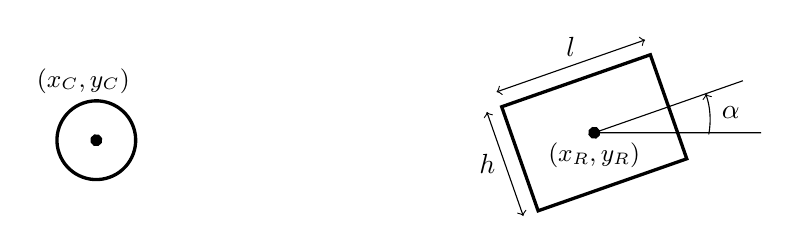
\begin{tikzpicture}
    \begin{scope}[rotate=19.29]
      \draw[very thick] (0, -.2) rectangle (2, 1.2) ;
      \draw[thin] (1, .5) -- ++ (2, 0) ;
      \draw[thin] (1, .5) -- ++ (2, -0.7) ;
      \draw[fill] (1, 0.5) circle (2pt) ;
      \draw[below] (1, 0.5) node {\small$(x_R, y_R)$} ;
      \draw[<->] (-.2, -.2) -- ++ (0, 1.4) ;
      \draw[left] (-.2, .5) node {$h$} ;
      \draw[<->] (0, 1.4) -- ++ (2, 0) ;
      \draw[above] (1, 1.4) node {$l$} ;
      \draw[<-] (2.5, 0.5) arc (0:-30:1) ;
      \draw[right] (2.5, .25) node {$\alpha$} ;
      \draw[very thick] (-5, 2.5) circle (.5) ;
      \draw[fill] (-5, 2.5) circle (2pt) ;
      \draw[above] (-5, 3) node {\small$(x_C, y_C)$} ;
    \end{scope}
  \end{tikzpicture}
\end{center}

Nous allons effectuer un changement de repère : l'origine du nouveau repère est le centre du rectangle est son orientation celle de la largeur du rectangle (c'est-à-dire une rotation de $-\alpha$). Le centre du cercle a pour coordonnées $(x'_C, y'_C)$ dans ce nouveau repère.

\begin{center}
  \begin{tikzpicture}
    \begin{scope}
      \draw[very thick] (0, -.2) rectangle (2, 1.2) ;
      \draw[fill] (1, 0.5) circle (2pt) ;
      \draw[below] (1, 0.5) node {\small$(0, 0)$} ;
      \draw[<->] (-.2, -.2) -- ++ (0, 1.4) ;
      \draw[left] (-.2, .5) node {$h$} ;
      \draw[<->] (0, 1.4) -- ++ (2, 0) ;
      \draw[above] (1, 1.4) node {$l$} ;
      \draw[very thick] (-5, 2.5) circle (.5) ;
      \draw[fill] (-5, 2.5) circle (2pt) ;
      \draw[above] (-5, 3) node {\small$(x'_C, y'_C)$} ;
    \end{scope}
  \end{tikzpicture}
\end{center}


Le calcul de $(x'_C, y'_C)$ (en fait $(Xcercle, Ycercle)$) est le suivant~:

\begin{lstlisting}
  let rectHalfWidth  = inRectangleSize.width  / 2.0
  let rectHalfHeight = inRectangleSize.height / 2.0
  let Xrelative = inCircleCenter.x - inRectangleCenter.x
  let Yrelative = inCircleCenter.y - inRectangleCenter.y
  let cosAngleRectangle = cos (inRectangleAngleInRadians)
  let sinAngleRectangle = sin (inRectangleAngleInRadians)
  let Xcercle =   Xrelative * cosAngleRectangle + Yrelative * sinAngleRectangle
  let Ycercle = - Xrelative * sinAngleRectangle + Yrelative * cosAngleRectangle
\end{lstlisting}

Comme on s'intéresse uniquement à vérifier que la distance cercle / rectangle est suffisante, on prend la valeur absolue de chaque coordonnée du centre du cercle~: on se ramène uniquement au premier quadrant.

\begin{center}
  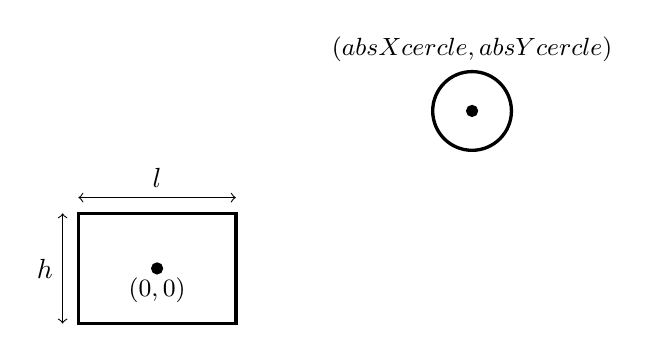
\begin{tikzpicture}
    \begin{scope}
      \draw[very thick] (0, -.2) rectangle (2, 1.2) ;
      \draw[fill] (1, 0.5) circle (2pt) ;
      \draw[below] (1, 0.5) node {\small$(0, 0)$} ;
      \draw[<->] (-.2, -.2) -- ++ (0, 1.4) ;
      \draw[left] (-.2, .5) node {$h$} ;
      \draw[<->] (0, 1.4) -- ++ (2, 0) ;
      \draw[above] (1, 1.4) node {$l$} ;
      \draw[very thick] (5, 2.5) circle (.5) ;
      \draw[fill] (5, 2.5) circle (2pt) ;
      \draw[above] (5, 3) node {\small$(absXcercle, absYcercle)$} ;
    \end{scope}
  \end{tikzpicture}
\end{center}


Ainsi : 
\begin{lstlisting}
  let absXcercle = fabs (Xcercle)
  let absYcercle = fabs (Ycercle)
\end{lstlisting}

La distance est suffisante si le centre du cercle se trouve \emph{au dessus} ou \emph{à droite} de la ligne $ABCD$.

\begin{center}
  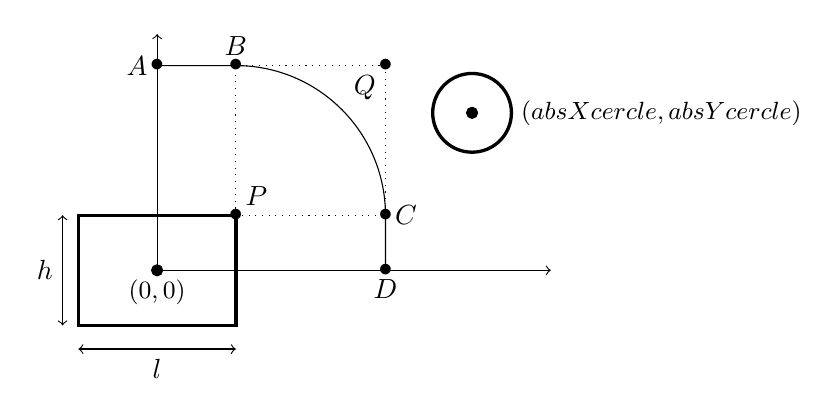
\begin{tikzpicture}
      \draw[very thick] (0, -.2) rectangle (2, 1.2) ;
      \draw[fill] (1, 0.5) circle (2pt) ;
      \draw[below] (1, 0.5) node {\small$(0, 0)$} ;
      \draw[<->] (-.2, -.2) -- ++ (0, 1.4) ;
      \draw[left] (-.2, .5) node {$h$} ;
      \draw[<->] (0, -.5) -- ++ (2, 0) ;
      \draw[below] (1, -.5) node {$l$} ;
    %--- Cercle
      \draw[very thick] (5, 2.5) circle (.5) ;
      \draw[fill] (5, 2.5) circle (2pt) ;
      \draw[above] (5.5, 2.5) node[right] {\small$(absXcercle, absYcercle)$} ;
      \draw[->] (1, 0.5) -- ++ (5, 0) ;
      \draw[->] (1, 0.5) -- ++ (0, 3) ;
    %--- Ligne ABCD
      \draw (1, 3.1) node {$\bullet$} node[left] {$A$}
         -- ++ (1, 0) node {$\bullet$} node[above] {$B$}
         arc (90:0:1.9) node {$\bullet$} node[right] {$C$}
         -- ++ (0, -.7) node {$\bullet$}  node[below] {$D$} ;
      \draw[dotted] (2, 1.2) node {$\bullet$} node[above right] {$P$}
        rectangle ++ (1.9, 1.9) node {$\bullet$} node[below left] {$Q$} ;
  \end{tikzpicture}
\end{center}

L'ordonnée des points $A$ et $B$ est $ h / 2 + r + iso$. L'abscisse des points $C$ et $D$ est $ l / 2 + r + iso$. $BC$ est un quart de cercle de centre le sommet supérieur droit du rectangle $P$, et de rayon $r + iso$.

L'isolation est respectée si :
\begin{itemize}
  \item le centre du cercle est \emph{suffisament} à droite ;
  \item ou \emph{suffisament} haut ;
  \item ou si il est dans la surface délimitée par $BQC$.
\end{itemize}

Le centre du cercle est \emph{suffisament} à droite~:
\begin{lstlisting}
  var ok = absXcercle >= (l / 2.0 + r + iso)
\end{lstlisting}


Le centre du cercle est \emph{suffisament} haut~:
\begin{lstlisting}
  if !ok {
    ok = absYcercle >= (h / 2.0 + r + iso)
  }
\end{lstlisting}

Le centre du cercle est est dans le rectangle $BPCQ$ et la surface délimitée par $BQC$
\begin{lstlisting}
  if !ok && (absXcercle >= (l / 2.0)) && (absYcercle >= (h / 2.0)) {
    let dx = absXcercle - l / 2.0
    let dy = absYcercle - h / 2.0
    let distance = sqrt (dx * dx + dy * dy)
    ok = distance >= (r + iso)
  }
\end{lstlisting}
